\section{Motivation}
\label{sec:motivation}

Takin as example a survay published by the U.S. Department of Commerce in 2020, the maintenance expenditure of the manufacturing industry in the United States were \$57.3 billion, while the losses due to preventable maintenance issues amounted to \$119.1 billion. The top 25 \% of those 
establishments relying on reactive maintenance was associated with 3.3 times more downtime 
than those in the bottom 25 \% \cite{NIST}. This means that the economic impact of failures exceeds the cost of maintenance by a factor of 2.1, and this is concentrated on those sectors that rely more on reactive maintenance.

In the article \cite{Maintenance_cat}, the authors divide the \gls{cbm} strategies in five categories:
\begin{itemize}
    \item Experience-based 
\end{itemize}

\begin{figure}
    \centering
    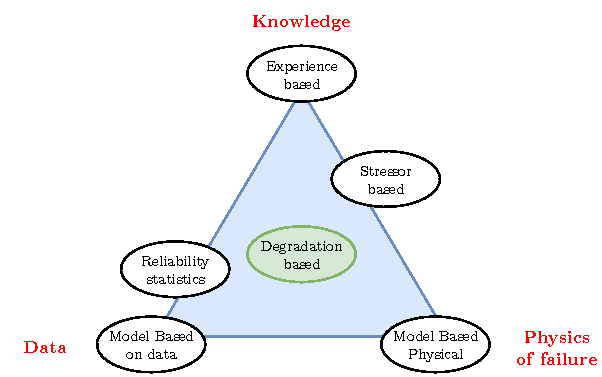
\includegraphics[scale=1.3]{images/Intro/MaintTriangle.pdf}
    \caption{Maintenance triangle \cite{Maintenance_cat}}
    \label{fig:MaintTriangle}
\end{figure} 